\chapter{Encoding Natural Deduction more faithfully}
\label{chap:I2L}

There are a lot of things wrong with the Natural Deduction encoding of \chapref{ItL}. Though it seems to allow forward and backward steps, in fact it breaks the rules of box-and-line displays. Its var/inscope mechanism isn't part of the logic it purports to imitate. Its error messages are phrased in terms of the sequent calculus, which its intended users --- students taking the logic course at QMW --- never saw. You could only make a single formula selection though some of the rules used in forward steps --- → elimination, ¬ elimination, ∀ elimination --- have more than a single antecedent and seemed naturally to need two. Worst of all, so far as novices are concerned, it allows metalogical steps involving unknowns, `incomplete' logical steps that have to be completed by subformula selection and unification.

Some of these problems were known to me. Some were revealed as the result of a research project looking at the r\^{o}le of visualisation in learning proofs. In one harrowing episode recorded on video, an incomplete ∀ intro step in a fairly straightforward proof reduced a student to tears of incomprehension and frustration. 

I fixed as many of these problems as I could, as well as I could. I'd be dishonest to claim that this encoding shows Jape's flexibility, because I had to modify its internal mechanisms quite a bit. But the mechanisms I provided are now available to all and with the exception of the Kripke-tree disproof mechanism (see next chapter), they are probably of general interest.

The encoding is in \textj{examples/naturaldeduction}, in file \textj{I2L.jt}.

\section{Rules}

The rules of this encoding are similar to those of \chapref{ItL}, except for `actual' in place of `var' and `inscope', and use of contradiction and truth symbols.
\begin{japeish}
RULE "→ elim"       IS FROM A→B AND A INFER B \\
RULE "∧ elim(L)"    IS FROM A ∧ B INFER A \\
RULE "∧ elim(R)"    IS FROM A ∧ B INFER B \\
RULE "∨ elim"       IS FROM A ∨ B AND A ⊢ C AND B ⊢ C INFER C \\
RULE "∀ elim"       IS FROM ∀x. P(x) AND actual i INFER P(i) \\
RULE "∃ elim"(OBJECT i) WHERE FRESH i AND i NOTIN ∃x.P(x) \\
                    IS FROM ∃x.P(x) AND actual i, P(i) ⊢ C INFER C \\
 \\
RULE "→ intro"          IS FROM A ⊢ B INFER A→B \\
RULE "∧ intro"          IS FROM A AND B INFER A ∧ B \\
RULE "∨ intro(L)"(B)    IS FROM A INFER A ∨ B \\
RULE "∨ intro(R)"(B)    IS FROM A INFER B ∨ A \\
RULE "¬ intro"          IS FROM A ⊢ ⊥ INFER ¬A \\
RULE "¬ elim"(B)        IS FROM B AND ¬B INFER ⊥ \\
RULE "∀ intro"(OBJECT i) WHERE FRESH i \\
                        IS FROM actual i ⊢ P(i) INFER ∀x .P(x) \\
RULE "∃ intro"          IS FROM P(i) AND actual i INFER ∃x.P(x) \\
 \\
RULE "contra (classical)"    IS FROM ¬A ⊢ ⊥ INFER A \\
RULE "contra (constructive)" IS FROM ⊥ INFER B \\
RULE "truth"                 IS INFER  ⊤ \\
 \\
RULE hyp(A) IS INFER A ⊢ A
\end{japeish}

These rules are more pronounceable than those of \chapref{ItL} --- elim and intro rather than -E and -I --- and they are organised into Forward and Backward menus. Although it is possible to run any rule backward, and most of them can be run forward with a bit of ingenuity, I put elim rules in the Forward menu, intro rules in Backward, and restricted cross-membership. The menu entries are labelled to give a hint of the effect of the step (and, in some cases, how to apply it).
\begin{japeish}
MENU Forward IS \\
\tab ENTRY   "∧ elim (preserving left)" ... \\
\tab ENTRY   "∧ elim (preserving right)" ... \\
\tab ENTRY   "→ elim"  ... \\
\tab ENTRY   "∨ elim (makes assumptions)" ... \\
\tab ENTRY   "¬ elim" ... \\
\tab ENTRY   "∀ elim (needs variable)" ... \\
\tab ENTRY   "∃ elim (assumption \& variable)" ... \\
\tab ENTRY   "contra (constructive)" ... \\
\tab SEPARATOR \\
\tab ENTRY   "∧ intro" ... \\
\tab ENTRY   "∨ intro (invents right)" ... \\
\tab ENTRY   "∨ intro (invents left)" ... \\
\tab SEPARATOR \\
\tab ENTRY   hyp ... \\
END

\end{japeish}
\begin{japeish}
MENU Backward IS \\
\tab ENTRY   "∧ intro" ... \\
\tab ENTRY   "→ intro (makes assumption)" ... \\
\tab ENTRY   "∨ intro (preserving left)" ... \\
\tab ENTRY   "∨ intro (preserving right)" ... \\
\tab ENTRY   "¬ intro (makes assumption A)" ... \\
\tab ENTRY   "∀ intro (introduces variable)" ... \\
\tab ENTRY   "∃ intro (needs variable)" ... \\
\tab ENTRY "truth" ... \\
\tab SEPARATOR\\
\tab ENTRY   "contra (classical; makes assumption ¬A)" ... \\
\tab ENTRY   "contra (constructive)"  ... \\
\tab ENTRY   "¬ elim (invents formulae)" ... \\
\tab SEPARATOR\\
\tab ENTRY   hyp ... \\
END
\end{japeish}
This is part of the push to make the logic more novice-accessible. But there's far more to it than that ...

\begin{figure}
\centering
\subfigure[∧ intro splits tree]{\centering
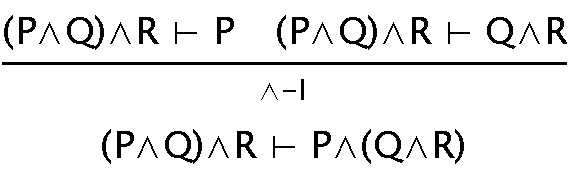
\includegraphics[scale=0.5]{pics/I2L/andintrotreeA}\label{fig:I2L:andintrotreeA}}
\qquad
\subfigure[expansion in one subtree]{\centering
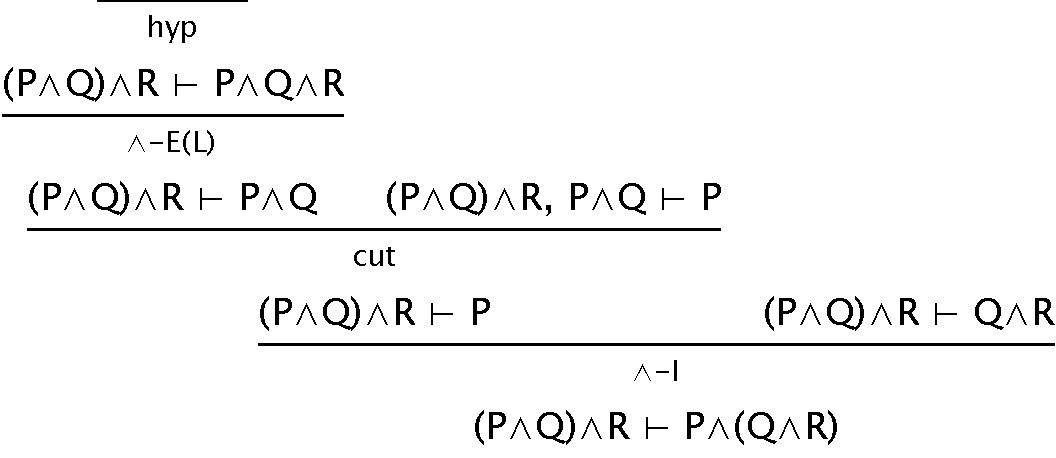
\includegraphics[scale=0.5]{pics/I2L/andintrotreeB}\label{fig:I2L:andintrotreeB}}
\caption{Separate subtrees have separate deductions}
\label{fig:I2L:andintrotree}
\end{figure}

\begin{figure}
\centering
\subfigure[faithful-looking box-and-line  rendering]{\centering
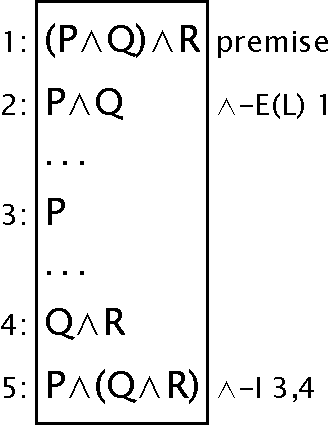
\includegraphics[scale=0.5]{pics/I2L/andintroboxB1}\label{fig:I2L:andintroboxB1}}
\qquad
\subfigure[is in fact a betrayal]{\centering
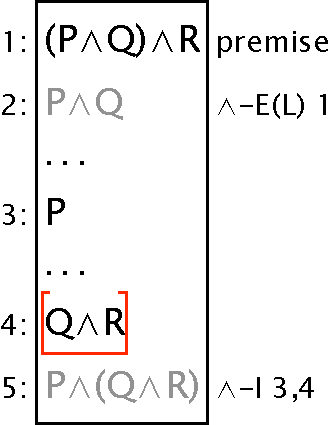
\includegraphics[scale=0.5]{pics/I2L/andintroboxB2}\label{fig:I2L:andintroboxB2}}
\caption{Separate subtrees affect the box-and-line display}
\label{fig:I2L:andintroboxB}
\end{figure}

\begin{figure}
\centering
\subfigure[elimination before introduction delays bifurcation]{\centering
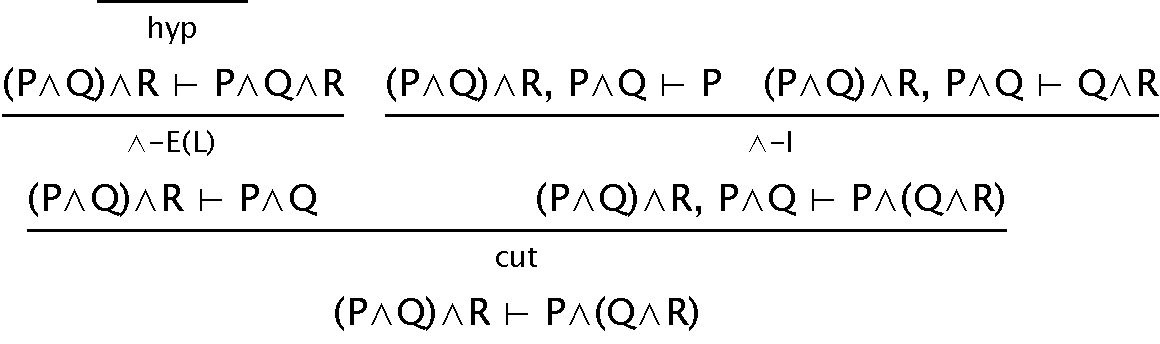
\includegraphics[scale=0.5]{pics/I2L/andintrotreeC}\label{fig:I2L:andintrotreeC}}
\qquad
\subfigure[and gives a more accurate box-and-line version]{\centering
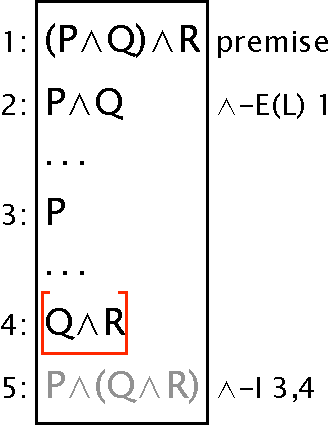
\includegraphics[scale=0.5]{pics/I2L/andintroboxC1}\label{fig:I2L:andintroboxC1}}
\caption{Separate subtrees force users to order their actions}
\label{fig:I2L:andintrotreeCC}
\end{figure}

\section{\textsc{cutin}: full-featured box-and-line steps}

The most glaring problem with the encodings that use box-and-line displays, before the advances discussed here, was that Jape broke the box-and-line rules. A simple ∧ introduction in the \chapref{ItL} encoding, for example, generates a bifurcated tree like that in \figref{I2L:andintrotreeA}. Any steps made in the left-hand subtree necessarily cannot be exploited in the right, and since all steps in this encoding take places at a tip of the tree, steps must be made in one or ther other. Suppose, for example, that the next step in the proof is an ∧ elim in the left subtree: the result is the tree in \figref{I2L:andintrotreeB}. Rendered in box-and-line form this gives \figref{I2L:andintroboxB1}. The display looks fine, but clicking on line 4 in \figref{I2L:andintroboxB2} reveals that it is not: line 1 is greyed out, inaccessible even though by box-and-line rules it can be used at line 4. That's not the only problem: although line 3 is black, it isn't available as a hypothesis selection in a proof of line 4. (Line 3 is an alternative conclusion, not greyed-out because you could select it instead of line 4. It looks just like a hypothesis, and this is very confusing to a novice who's been taught the basic rule of box-and-line proof, that lines above you and not inside a protecting box can always be called upon.)

That's not all. The tree in \figref{I2L:andintrotreeC} is what you get if you do the ∧ elimination first, then the introduction. It gives \emph{exactly the same} box-and-line display, but this time (\figref{I2L:andintroboxC1}) line 1 is accessible from everywhere. The order in which you make steps is important, even though it doesn't show immediately in the box-and-line display. 

It's surely obvious that in a box-and-line proof you ought to be able to make forward and backward steps in whatever order you like, and that lines which look as if they could be used as hypotheses can be used as hypotheses. That's hard when the underlying structure is a proof tree. The obvious fix would have been to rework Jape to use a box-and-line structure as its underlying proof structure, but I didn't have the time to do that nor did I have any idea how to solve the difficulties that I could foresee in such a treatment. Instead I discovered how to fix the problem, somewhat laboriously, within the Jape tree. So far as forward steps are concerned, the basic idea is that cut nodes can be inserted into the tree: i.e. a tree like \figref{I2L:andintrotreeA} can be transformed into one like \figref{I2L:andintrotreeC} by a step of ∧ elimination (see \secref{I2L:forwardCUTIN}).

The \textsc{cutin} tactic takes a subtree (not necessarily a tip, not necessarily the root of the current tree)
\begin{equation*}
\cols[c]\vdots\\\Gamma|-C\sloc
\end{equation*}
inserts an extra left-hand-side formula $B$  and makes the result the right antecedent of a cut step, producing the new subtree
\begin{equation*}
\infer{\Gamma|-C}{\cols[c]\vdots\\\Gamma|-B\sloc & \cols[c]\vdots\\\Gamma,B|-C\sloc}
\end{equation*}
Then it runs a tactic in the left antecedent of the cut step. Finally it returns to the position in the now-modified right antecedent at which it was originally applied.

Inserting a cut node in this way means putting an extra left-hand-side formula in every sequent of the modified subtree, and  that means, in some cases, generating extra \textsc{notin} provisos if the tree contains steps that used \textsc{fresh}. Jape can only do it if the logic has a cut rule that is the right shape, and if the rules are stated additively without mentioning contexts explicitly --- that is, \textj{autoadditiveleft} is set true --- so that extra left-hand formulae can be inserted freely.

Since the intention is to overcome the effects of bifurcating rules like ∧ intro, it's easiest to begin by discussing how \textsc{cutin} can be used with backward rules.

\begin{figure}
\centering
\subfigure[line 1 is always a hypothesis]{\centering
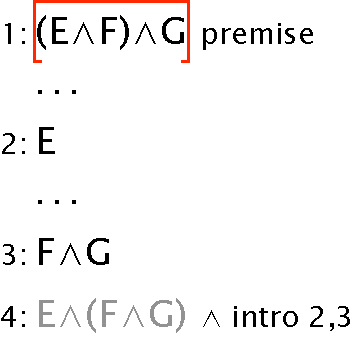
\includegraphics[scale=0.5]{pics/I2L/andcutinboxA}\label{fig:I2L:andcutinboxA}}
\qquad
\subfigure[line 3 is always a conclusion]{\centering
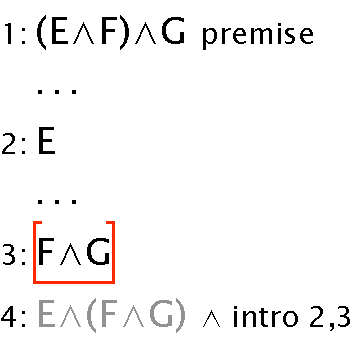
\includegraphics[scale=0.5]{pics/I2L/andcutinboxB}\label{fig:I2L: andcutinboxB}}
\qquad
\subfigure[line 2 can be a hypothesis]{\centering
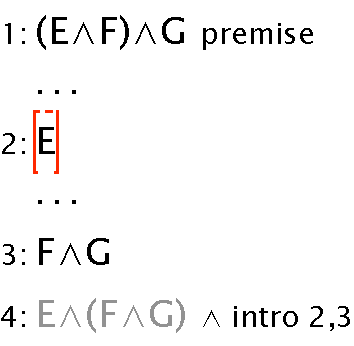
\includegraphics[scale=0.5]{pics/I2L/andcutinboxC}\label{fig:I2L: andcutinboxC}}
\qquad
\subfigure[line 2 can also be a conclusion]{\centering
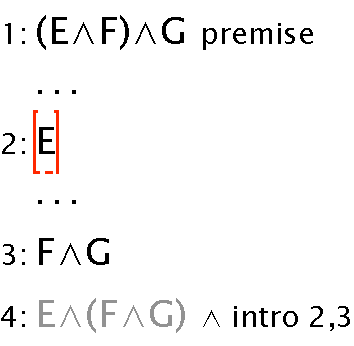
\includegraphics[scale=0.5]{pics/I2L/andcutinboxD}\label{fig:I2L: andcutinboxD}}
\caption{Visible components in an accurate box-and-line display}
\label{fig:I2L:andcutinbox}
\end{figure}

\begin{figure}
\centering
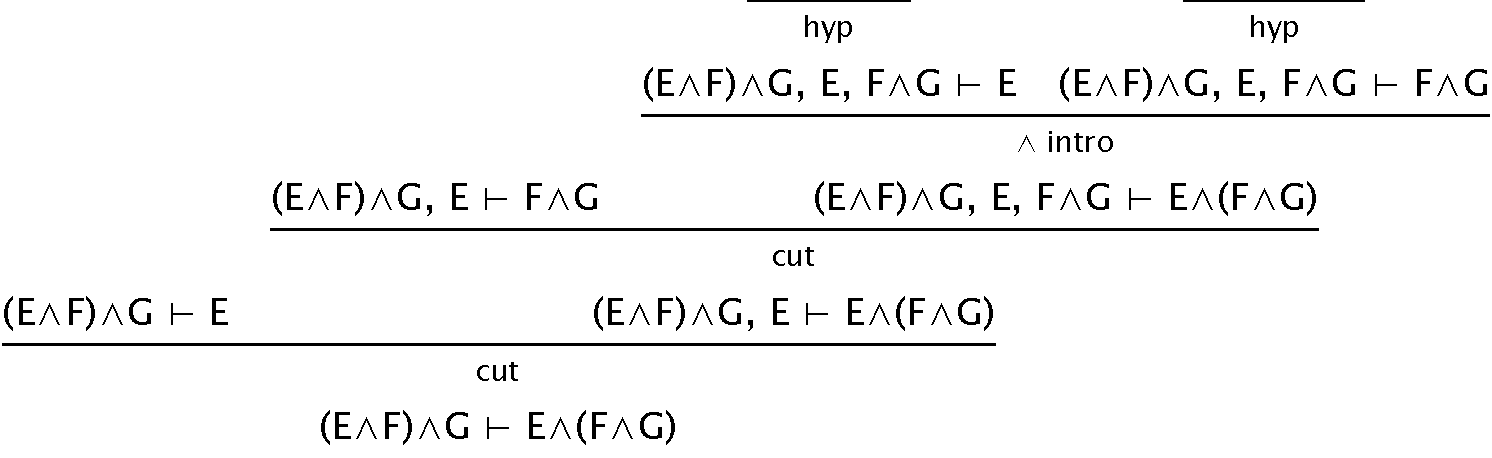
\includegraphics[scale=0.5]{pics/I2L/andcutintree}
\caption{∧ intro generates two cut nodes}
\label{fig:I2L:andcutintree}
\end{figure}

\subsection{\textsc{cutin} and backward steps}

\Figref{I2L:andcutinbox} shows the various selections that can be made after a backwards ∧ intro step in the encoding of this chapter. Lines 1 and 3 have a fixed interpretation as hypothesis and conclusion respectively. Line 2, intermediate between the two, needs proof but, according to the rules of box-and-line proofs, can also be called upon if necessary in the proof of line 3. In this encoding it can: different ways of clicking on the line select it as hypothesis or conclusion (see \secref{I2L:formulaselection}). 

The magic is done with a couple of cuts, as shown in \figref{I2L:andcutintree}: $E$ and $F@G$ are inserted as hypotheses, and the actual ∧ intro proof step closed with hyp. The effect is that the tip conclusion $F@G$ can see the hypothesis $E$. The box-and-line translation, and the selection mechanism, had to be modified to deal with intermediate lines like line 3. The \textsc{goalpath} navigation mechanism had to be modified to deal specially with cut nodes that can be inserted after a path has been recorded (I'm inordinately proud of the fact that I got that bit to work, but it would be a mistake to try to describe its intricacy here). Otherwise it's all down to \textsc{cutin}.

\textsc{Cutin} in backward steps is usually applied via the fstep tactic. The menu entry for ∧ intro, stripped of its error-handling protection (I'll come back to that) is essentially
\begin{japeish}
SEQ "∧ intro" fstep fstep
\end{japeish}
(see "∧ intro backward" in \textj{I2L\_menus.j}). "∧ intro" is the Natural Deduction rule --- see \textj{I2L\_rules.j}
\begin{japeish}
RULE "∧ intro" IS FROM A AND B INFER A ∧ B
\end{japeish}
--- which generates two open subgoals. Fstep takes an open goal, \textsc{cutin}s its conclusion as a hypothesis, and closes the original goal with hyp. It's in \textj{examples/forwardsteptechnology/forwardstep.j} along with the trueforward tactic which it calls upon:
\begin{japeish}
TACTIC fstep IS \\
\tab ALT \\
\tab \tab (ANY (MATCH hyp)) \\
\tab \tab (trueforward SKIP) \\
\\
MACRO trueforward(tac) IS \\
\tab LETGOAL \_A \\
\tab \tab (CUTIN (LETGOAL \_B (UNIFY \_A \_B) tac)) \\
\tab \tab (ANY (MATCH hyp))
\end{japeish}
Fstep tries to match the open goal with any left-hand-side formula so as to avoid unnecessary duplication of hypotheses (no unification allowed: this must be done without changing the values of any unknowns in the proof tree). If that fails it applies trueforward \textsc{skip}. Trueforward records the current goal (\textsc{letgoal} \_A) and then does a \textsc{cutin}. \textsc{Cutin} looks for the correct place to cut the tree: it's the lowest point below the current node which has the same left-hand-side formulae as the current node, i.e. the lowest place in the tree, and therefore the highest place in the box-and-line display, where all the currently visible hypothesis lines are available. It runs its argument on the left-hand-side of the cut node it inserts there: in this case it records the new goal --- the cut formula, which is also the inserted hypothesis on the right-hand-side of the cut node --- in \_B and unifies it with \_A. Then it runs tac, which in this case is \textsc{skip}, and \textsc{cutin} is finished. Finally, back at the original open goal but now in the new subtree, hyp matches with the hypothesis that must now be there. Apply all that twice, as "∧ intro backward" does, and you get the effect shown in \figref{I2L:andcutintree}.

\begin{figure}
\centering
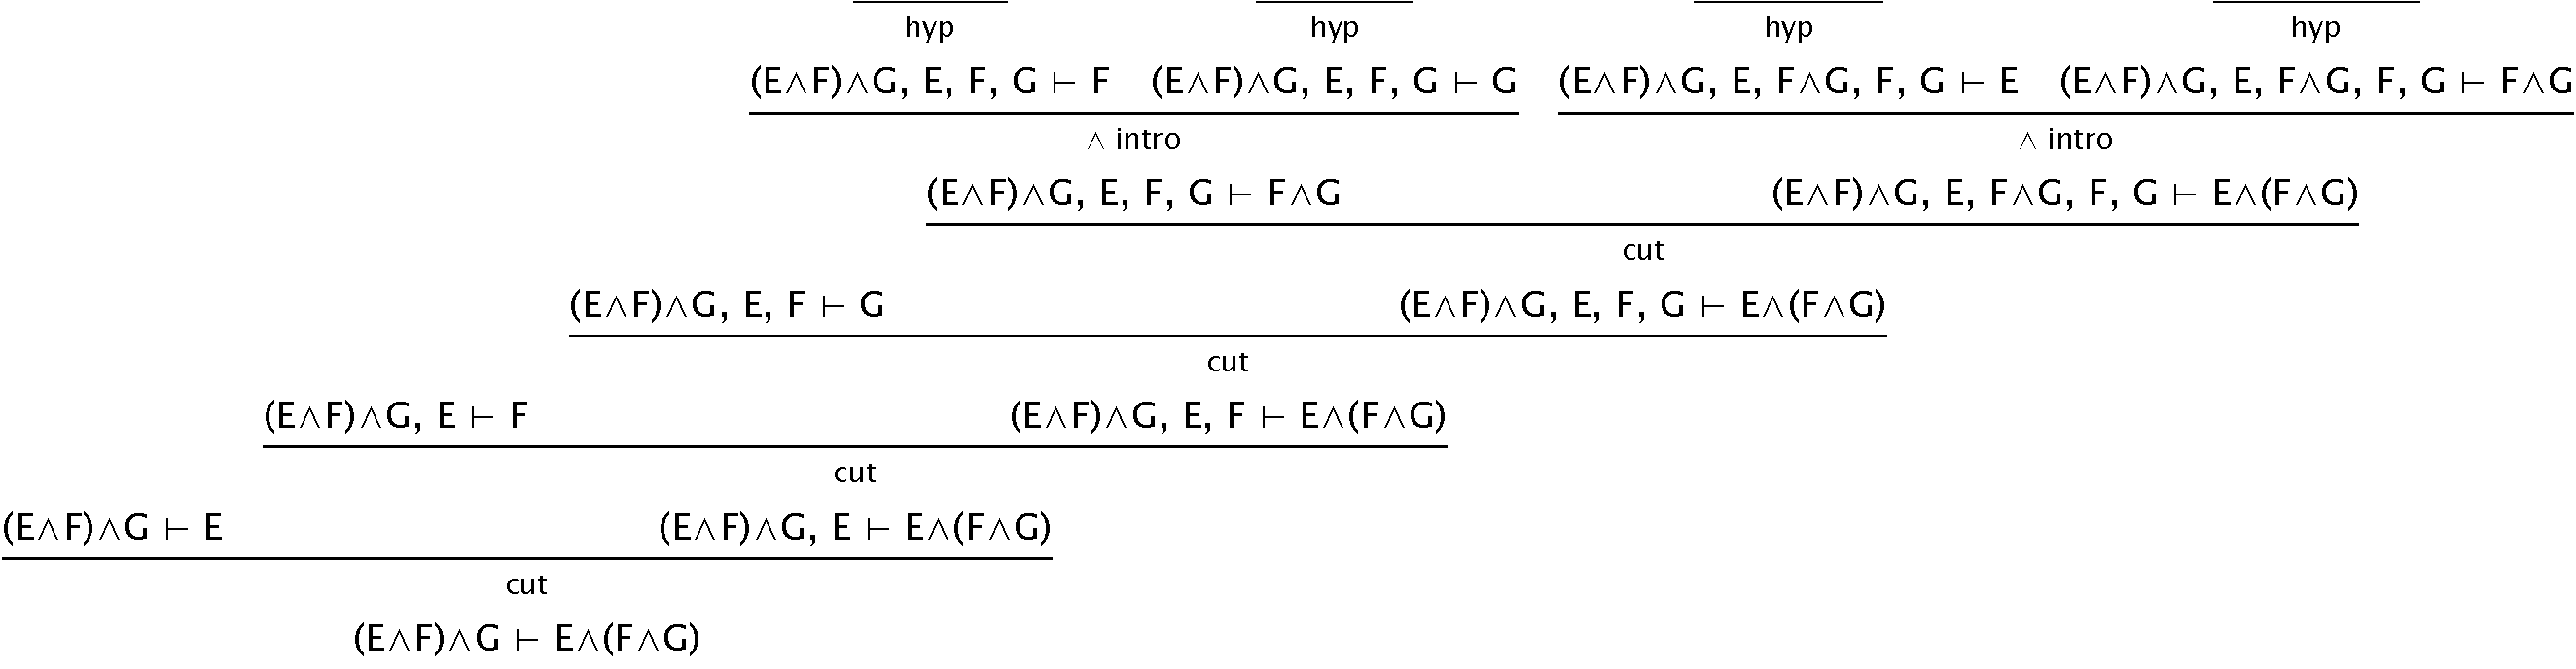
\includegraphics[scale=0.35]{pics/I2L/andcutintree2}
\caption{A second ∧ intro gives two more cut nodes}
\label{fig:I2L:andcutintree2}
\end{figure}

\begin{figure}
\centering
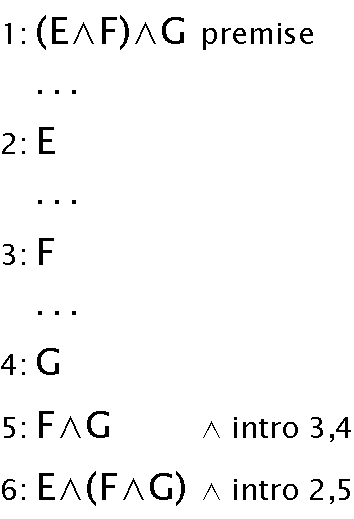
\includegraphics[scale=0.5]{pics/I2L/andcutinbox2}
\caption{A concise summary of \figref{I2L:andcutintree2}}
\label{fig:I2L:andcutinbox2}
\end{figure}

Want to see it again? \Figref{I2L:andcutintree2} shows the effect of applying ∧ intro again, this time to the $F@G$ tip. The \textsc{cutin} place in \figref{I2L:andcutintree} is the parent node of that tip, and anything in its right-hand subtree will be able to see the \textsc{cutin} formula. Once again, two cut nodes; once again, the actual proof step closed by hyp; once again, the cumbersome tree concisely summarised in box-and-line style (\figref{I2L:andcutinbox2}), this time with two more intermediate formulae on lines 2 and 3.

So much for backward steps: they work properly if they use fstep freely. To discuss how forward steps use \textsc{cutin}, it's first necessary to discuss formula selection.

\section{Formula selection}
\label{sec:I2L:formulaselection}

If you click on line 4 of \figref{I2L:andcutinbox2}, you are in effect clicking on the tip conclusion $G$ of the tree in \figref{I2L:andcutintree2}. That same click might be interpreted as selecting one of the left-hand-side occurrences of $G$ elsewhere in the tree, but those left-hand selections would be pointless, because they are all of hypotheses in a closed tree, with no open conclusion to which they might correspond. This was one part of the original treatment of cut nodes in box-and-line display: in that tree $G$ is only useful as a conclusion, so when you click on it it's obvious what you mean.

If you click on line 5, Jape rejects the attempt: you are pointing to $F@G$, which occurs only as a conclusion in a closed tree, at the root of a completed ∧ intro step. The same with line 6.

If you click on line 1, it's clear that $(E@F)@G$ occurs only as a left-hand-side formula, but it occurs at every node of the tree. The canonical instance --- the one that generates line 1 --- is at the root of the tree, so Jape regards that as the location of the selection. If you then conclusion-click on some other line --- line 3, for example --- the two selections are regarded as taking place in the $(E@F)@G, E |- F$ tip. This is the original treatment of hypothesis + conclusion selections in box-and-line displays.

Before \textsc{cutin}, all operations on a tree happened at tips, and a click on line 1 of \figref{I2L:andcutinbox2} was by itself ambiguous, because it indicated the root of a tree with three tips ($E$, $F$ and $G$). Until this encoding it was regarded as incomplete: ``There is more than one unproved conclusion'', Jape used to complain; ``Please select the one you want to work on''. But now we can apply a \textsc{cutin} step anywhere in the tree, so \textj{I2L\_settings.j} contains
\begin{japeish}
INITIALISE seektipselection false
\end{japeish}
and Jape no longer complains about selections that don't describe tip nodes. You can still tell if the selection is at a tip, because \textsc{letgoal} can only match at a tip (\textsc{letrhs} matches at any node of the tree provided there's a single conclusion formula).

$F$ on line 3 is more of a problem. It occurs at a tip in \figref{I2L:andcutintree2}, but it also occurs as a left-hand-side formula in a tree that isn't closed. So it might be used as a conclusion, or it might be used as a hypothesis somehow to prove $G$, the only tip in that tree. In the box-and-line display it can be seen as intermediate between lines 1 and 2, a bridge between them. A click on an intermediate line is by itself ambiguous, and such lines are now treated specially. A click in the upper half of the formula produces a selection open towards the top -- a conclusion selection, indicating the tip occurrence -- and a click in the lower half is a hypothesis selection indicating the occurrence as a left-hand-side formula.

To summarise: a conclusion-click selects a right-hand-side formula at a tip; a hypothesis-click gives you the original left-hand-side occurrence of the formula. This isn't new --- it's the way that clicks always worked --- but the possibility of accepting a selection outcome which isn't at a tip is new, as is the way of selecting different readings of ambiguous lines.

\subsection{Forward steps with \textsc{cutin}}
\label{sec:I2L:forwardCUTIN}

Given a non-tip selection like line 1 of \figref{I2L:andcutinbox2}, a step from the Forward menu invokes (after some checking for errors) ForwardCut in \textj{I2L\_menus.j}
\begin{japeish}
TACTIC ForwardCut (n,rule) IS CUTIN (ForwardUncut n rule)
\end{japeish}
and the part of ForwardUncut that matters is
\begin{japeish}
LETHYP \_Ah \\
\tab (LETGOALPATH G \\
\tab \tab (WITHARGSEL Rule) \\
\tab \tab (GOALPATH (SUBGOAL G n)) \\
\tab \tab (WITHHYPSEL hyp) \\
\tab \tab (GOALPATH G) \\
\tab \tab NEXTGOAL)
\end{japeish}
--- apply the rule to the left antecedent of the cut produced by \textsc{cutin}, go to its $n$th antecedent, apply hyp to match the selection, then go back to the root of the left antecedent and look for the next goal. In the ForwardCut use that last bit doesn't matter, because \textsc{cutin} returns to the original application position. (And in any case I don't use \textj{autoselect}: the user must always indicate, by selection, where to work next. I think the \textsc{nextgoal} stuff is inherited from some other encoding.)

The second alternative in ForwardUncut deals with the possibility that it's applied without a hypothesis selection: that can happen if there is only one hypothesis formula in the tree. \textsc{Letlhs} \_Ah matches just if there is a single left-hand-side formula; what follows imitates what happens with a hypothesis selection.
\begin{japeish}
LETLHS \_Ah \\
\tab (LETGOALPATH G \\
\tab \tab (WITHARGSEL Rule)\\
\tab \tab (GOALPATH (SUBGOAL G n))\\
\tab \tab (LETGOAL \_Ag (UNIFY \_Ag \_Ah) (ANY hyp))\\
\tab \tab (GOALPATH G) \\
\tab \tab NEXTGOAL)
\end{japeish}
(The \textsc{unify} is used in case Rule introduces any new left-hand-side formulae. Making \_Ah an argument to hyp doesn't always work, for reasons which now escape me.)

\begin{figure}
\centering
\subfigure[selecting only line 1]{\centering
\makebox[150pt]{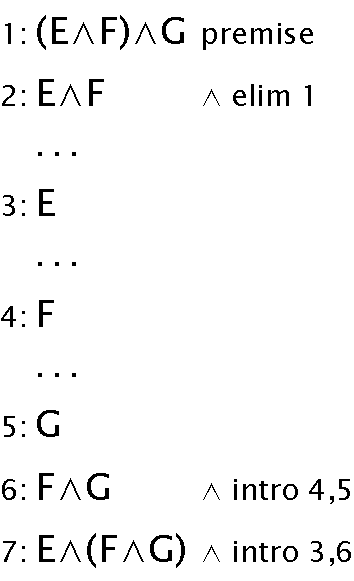
\includegraphics[scale=0.5]{pics/I2L/andcutinbox3A}}\label{fig:I2L:andcutinbox3A}}
\subfigure[selecting lines 1 and 4]{\centering
\makebox[150pt]{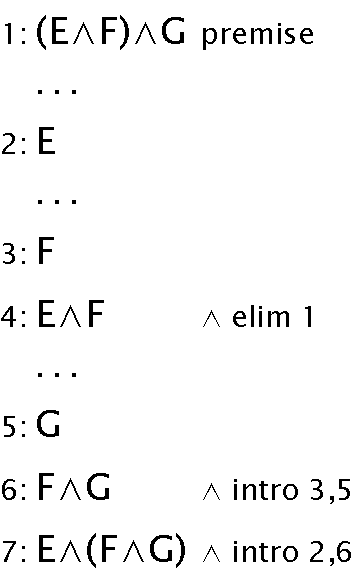
\includegraphics[scale=0.5]{pics/I2L/andcutinbox3B}}\label{fig:I2L:andcutinbox3B}}
\caption{∧ elim in \figref{I2L:andcutinbox2} after different selections}
\label{fig:I2L:andcutinbox3}
\end{figure} 

With a single selection of line 1 in \figref{I2L:andcutinbox2} a step of ∧ elim produces \figref{I2L:andcutinbox3A} because the cut is applied to the root of the tree in \figref{I2L:andcutintree2}, and the new left-hand-side formula, on line 2, is visible throughout all its right antecedent subtree. With a selection of line 1 and line 4, the cut is applied much higher up the tree, just below the $G$ tip, and the result is \figref{I2L:andcutinbox3B} where the new left-hand-side formula appears in the new line 4. (It's odd at first to realise that lower down the diagram means higher up the tree, but you get used to it.)

\section{Multiple hypothesis selections}

In the sequent calculi which Bernard and I initially encoded, a single left- or right-hand-side formula selection at a tip was enough to indicate the component that was to be worked on by a rule step. This led to a slogan: ``point at what you want to work on'', and a simple interaction mechanism. Later I had to modify it a bit to allow single hypothesis + single conclusion selections in the box-and-line display --- just because a single hypothesis line stands for a multiplicity of left-hand-side occurrences --- but we still stuck to single selections on either side of the sequent. Sometimes we smuggled extra hypothesis selections in by demanding a subformula selection, but the cure was worse than the disease, in UI design terms (it was lack of such a selection that reduced that videoed student to tears).

\begin{figure}
\centering
\subfigure[the problem]{\centering
\makebox[150pt]{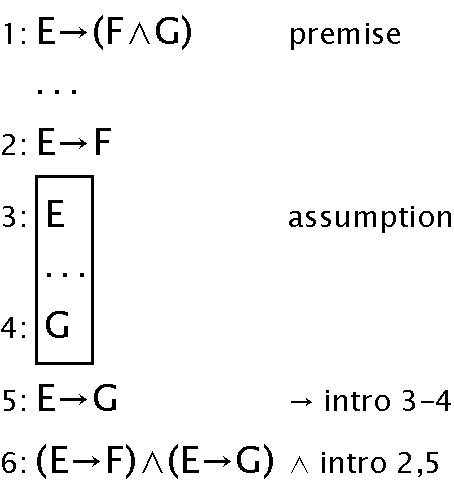
\includegraphics[scale=0.5]{pics/I2L/andelimbox1A}}\label{fig:I2L:andelimbox1A}}
\subfigure[lines 1 and 4 selected]{\centering
\makebox[150pt]{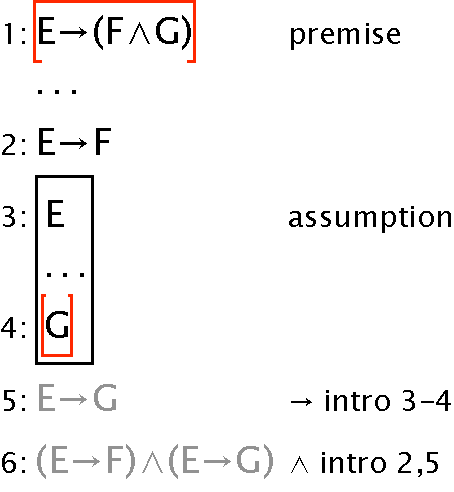
\includegraphics[scale=0.5]{pics/I2L/andelimbox1B}}\label{fig:I2L:andelimbox1B}}
\subfigure[lines 1 and 3 selected]{\centering
\makebox[150pt]{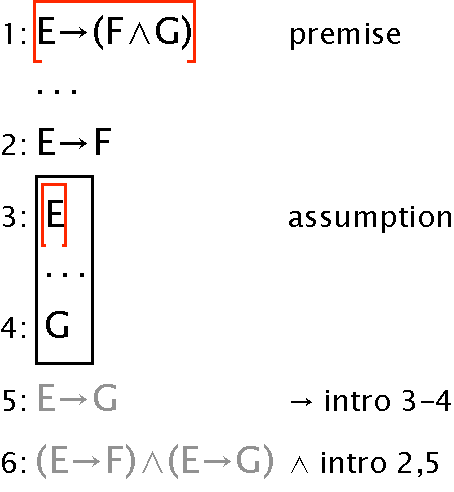
\includegraphics[scale=0.5]{pics/I2L/andelimbox1C}}\label{fig:I2L:andelimbox1C}}
\caption{∧ elim: advantages of multi-hypothesis selection}
\label{fig:I2L:andelimbox1}
\end{figure}

In Natural Deduction several rules used in forward steps --- → elim, ¬ elim and ∀ elim at least --- have more than one antecedent, and it's unreasonable to force your users to point at only one of them. Consider \figref{I2L:andelimbox1A}, for example. To make an ∧ elim step in the \chapref{ItL} encoding, you have to point at lines 1 and 4, as in \figref{I2L:andelimbox1B}. In the \textj{I2L.jt} encoding of this chapter, you click line 1, shift-click line 3 (or, of course, the other way round) as in \figref{I2L:andelimbox1C}. Much more natural, much easier to explain to a novice (especially with good error reporting: see \secref{I2L:errors}). 

Jape has two mechanisms to deal with multi-hypothesis selections. \textsc{Lethyps2} \textit{pat1} \textit{pat2} recognises exactly two selections; \textsc{lethyps} \textit{pat} recognises more than one selection (sorry!) and binds them as a tuple to \textit{pat}. (In this encoding \textsc{lethyps} is mostly used for error analysis, but it gets a bit more of an outing in \chapref{Hoare}.) The → elim menu entry in \textj{I2L\_menus.j} leads to the tactic
"→ elim forward", which has the structure
\begin{japeish}
TACTIC "→ elim forward" IS \\
\tab WHEN \\
\tab \tab (LETHYP2 \_A (\_A→\_B) ... normal ...) \\
\tab \tab (LETHYP2 \_C (\_A→\_B) ... error ...) \\
\tab \tab (LETHYP2 \_A \_B ...) \\
\tab \tab (LETHYP (\_A→\_B) \\
\tab \tab \tab (WHEN  \\
\tab \tab \tab \tab (LETCONC \_C ... accepted ...) \\
\tab \tab \tab \tab (... error ...))\\
\tab \tab (LETHYP \_A ... error ...)\\
\tab \tab (LETHYPS \_A ... error ...)\\
\tab \tab (...)
\end{japeish}
The first line recognises two hypothesis selections which match the antecedents of → elim (the order of selection doesn't matter). The second matches two selections which don't quite match: one of them is an → formula, but the other doesn't fit its right-hand side. The third alternative matches two hypothesis selections in which neither is an → formula. The fourth alternative matches a single selection which is an → formula: that's acceptable if there's also a conclusion selection (\textsc{letconc}), otherwise not.\footnote{The half-forward, half-backward step which allows us to deduce $B$ from $A->B$, preceding the deduction with an open conclusion $A$, is useful and I decided to permit it. But I insisted that there had to be a way of signalling that the user knew that just that step was being carried out.} The fifth alternative deals with a single selection which isn't an → formula. The sixth handles the case that there are more than two hypothesis selections. The last complains that there are no selections at all.\footnote{Other forward steps are allowed if there's only a single left-hand-side formula which matches the rule --- \textsc{letlhs} would check for that --- but in this case I thought it wasn't appropriate.}

The techniques used in the tactic are dealt with in the discussion of error checking and reporting (\secref{I2L:errors}).

\section{Only complete steps allowed}

One of the things that James Aczel's excoriating videos demonstrated to me was the difficulty students had with what he called 'incomplete steps'. Jape had been designed from the first to allow exploration, and in particular to insert unknowns if the user didn't or couldn't supply enough information to describe a definite instance of a rule step. 

\begin{figure}
\centering
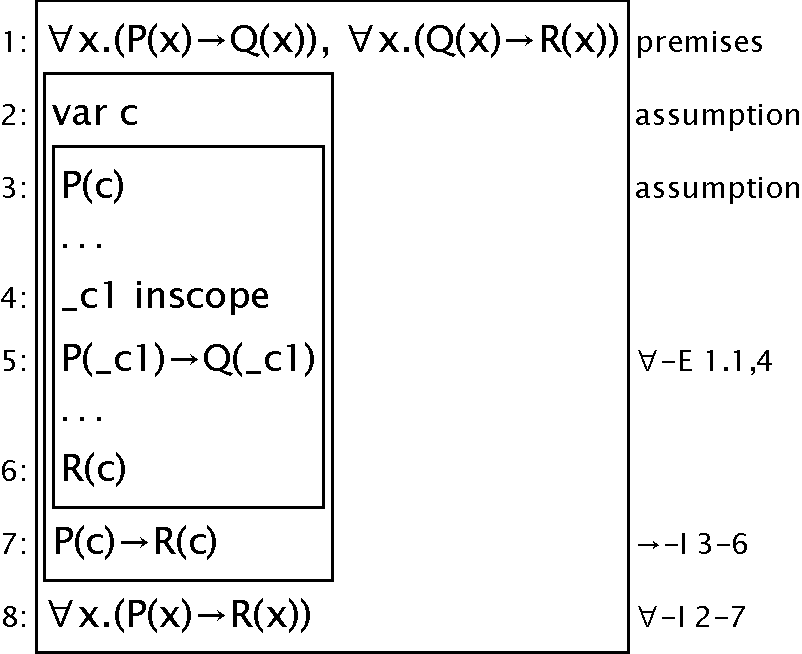
\includegraphics[scale=0.5]{pics/I2L/tearprovocation}
\caption{A tear-provoking, or fury-provoking, mis-step}
\label{fig:I2L:tearprovocation}
\end{figure}

The ∀ elimination step in the  \chapref{ItL} encoding, for example,
\begin{japeish}
RULE "∀-E"(c) IS FROM ∀x. A(x) AND c inscope INFER A(c)
\end{japeish}
might almost have been designed to generate incomplete steps. The `c inscope' antecedent was normally hidden. The rule was applied from the menu by the tactic
\begin{japeish}
TACTIC "∀-E with side condition hidden" IS \\
\tab LAYOUT "∀-E" (0) (WITHARGSEL "∀-E")
\end{japeish}
and there was a rule
\begin{japeish}
RULE "inscope" IS INFER var x ⊢ x inscope
\end{japeish}
which was applied automatically and silently, like hyp, before the effect of a user's action was displayed. The idea was that the user would subformula-select something to correspond to $c$ when applying the rule. (I realised at the time that I was in effect smuggling in an extra hypothesis selection, but I didn't realise what harm that could do.)

One tearful novice generated a proof display like that shown in \figref{I2L:tearprovocation} simply by making a ∀-E step without the necessary subformula selection of $c$ on line 2. The nonsense on line 4 was beyond her comprehension --- quite reasonably as I now see it --- and she couldn't see through that to realise that her problem was to pick something to match \_c1.

Aside from the var/inscope silliness in the \chapref{ItL} encoding, unknowns are useful tools, even essential tools. But to novices they are an intrusion, something that Jape uses but the logic doesn't, and they become a barrier to learning. When necessary (see \chapref{Hoare}) even novices must be able to deal with them, but then they take a bit of explaining. When unnecessary, as in this example, the logic designer must squirm with embarrassment. I squirmed.

After squirming, I took James's criticisms to heart and designed the new encoding to deny the possibility of incomplete steps. The flexibility that novices lose was in any case inaccessible to them while they were still struggling with the meaning of logic and the notion of proof search. ``Do it this way'' was a possible injunction and a useful one (users might not find out so much about what Jape can do, but so what?). 

The ∀ elimination step in the new encoding is
\begin{japeish}
RULE "∀ elim" IS FROM ∀x. P(x) AND actual i INFER P(i)
\end{japeish}
and it's applied by a tactic which requires that you select something for both antecedents:
\begin{japeish}
TACTIC "∀ elim forward" IS \\
\tab WHEN     \\
\tab \tab (LETHYP2 (actual \_i) (∀\_x.\_A) ... normal ...) \\
\tab \tab (LETHYP (∀\_x.\_A) ... not enough ...) \\
\tab \tab (LETHYP (actual \_i) ... not enough ...) \\
\tab \tab (LETHYPS \_As ... not correct ...) \\
\tab \tab (LETGOAL (∀\_x.\_A) ... perhaps ∀ intro is called for ...) \\
\tab \tab (... no selections ...)
\end{japeish}

That sort of thing, applied in every step, seems to be effective.\footnote{Nobody has yet conducted educational experiments to check this assertion. Volunteers welcome.} It's tedious and difficult, and it feels quite ad-hoc while you're doing it, but I don't know a better way. I can't imagine that there's a better way available within the architecture of Jape.

\section{Error checking and reporting}
\label{sec:I2L:errors}

One thing which James's videos impressed on me was the inutility of Jape's error messages. They were expressed in language which the students couldn't understand, talking of antecedents, goals, tips, and I don't know what else. Students responded by ignoring all error messages, which didn't help the learning experience. So I fixed the error messages. It was a lot of work, and it appeared to help.

\subsection{Enhanced alerts}

The \textsc{alert} tactic takes a variety of arguments.  The basic shape is
\begin{quote}
\textsc{alert} \textit{message} \textit{button} ...
\end{quote}
\textit{Message} describes the text of the alert. The simplest \textit{message} is a string, but there's also a \textj{printf}-style variation: a tuple of a string and arguments. Format specifiers in the string are expanded using the arguments: \%s for a string; \%t for a formula (a `term'); \%l for a `list' (actually a tuple: sorry). In the \%l case the argument can be ((t0,t1,...,tn), sep) or it can be ((t0,t1,...,tn), sep1, sep2): the first alternative gives you t0<sep>t1<sep>...<sep>tn; the second gives you t0<sep1>t1<sep1>...<sep2>tn. You can put newlines in the string with {\textbackslash}n.

Each \textit{button} is a pair of a button label (which is a \textit{message}) and a tactic. You get a button labelled with the label, which runs the tactic when you press it.

Here's an example:
\begin{japeish}
ALERT\\
\tab                "To make a ∀ elim step forward, you must select a hypothesis {\textbackslash} \\
\tab {\textbackslash}of the form ∀x.A, and also a pseudo-assumption of the form {\textbackslash}\\
\tab {\textbackslash}actual i. You didn't select any hypotheses, but the current {\textbackslash}\\
\tab {\textbackslash}conclusion is \%t, which could be used to make a ∀ intro step {\textbackslash}\\
\tab {\textbackslash}backwards.{\textbackslash}\\
\tab {\textbackslash}{\textbackslash}nDid you perhaps mean to make a backward step with {\textbackslash}\\
\tab {\textbackslash}∀ intro?", ∀\_x.\_A) \\
\tab ("OK",STOP) ("Huh?",SEQ Explainhypothesisandconclusionwords STOP)
\end{japeish}

\subsection{Careful step-checking}

Most of the work went into checking the way that rules are applied, and customising alerts for them. The tactic applied when you ask for ∧ intro, for example is
\begin{japeish}
BackwardOnlyC \\
\tab (QUOTE (\_A∧\_B)) (Noarg "∧ intro backward" "∧ intro") "∧ intro" "A∧B"
\end{japeish}
BackwardOnlyC checks that you are applying the step without any confusing hypothesis selection:
\begin{japeish}
TACTIC BackwardOnlyC (pattern, action, stepname, shape) IS\\
\tab BackwardOnly pattern action stepname shape \\
\tab \tab "can also be used forward -- see the Forward menu"
\end{japeish}
BackwardOnly (in \textj{backwardstep.j} in \textj{examples/backwardstep\_technology}) is
\begin{japeish}
MACRO BackwardOnly (pattern, action, stepname, shape, explain) IS \\
\tab WHEN \\
\tab \tab (LETGOAL pattern (BackwardOnly2 stepname action explain)) \\
\tab \tab (LETGOAL \_A (ComplainBackwardWrongGoal stepname shape)) \\
\tab \tab (ComplainBackward pattern stepname shape)
\end{japeish}
(it's a \textsc{macro} rather than a \textsc{tactic} because you don't want to evaluate the arguments, just use them). The first alternative tests that you are at a tip whose right-hand-side formula matches \_A∧\_B; if you are at some other kind of tip the second alternative generates a message; if you aren't at a tip it's the third alternative and an alternative message. (For details of what those messages are, look in \textj{explain\_selections.j} in \textj{examples/explain\_technology}.)

If you are at the right kind of tip, BackwardOnly2 checks that you haven't for some reason selected a hypothesis formula or two:
\begin{japeish}
TACTIC BackwardOnly2 (stepname, action, explain) IS \\
\tab WHEN \\
\tab \tab (LETHYPS \_Ahs \\
\tab \tab \tab (WHEN  \\
\tab \tab \tab \tab (LETCONC \_Ac \\
\tab \tab \tab \tab \tab (BackwardOnly3 stepname action explain \_Ahs \_Ac ", selecting"))  \\
\tab \tab \tab \tab (LETRHS \_Ac  /* can't fail */  \\
\tab \tab \tab \tab \tab (BackwardOnly3 stepname action explain \_Ahs \_Ac " from"))))  \\
\tab \tab (WITHSELECTIONS action)
\end{japeish}
The second alternative applies the original action 
\begin{japeish}
Noarg "∧ intro backward" "∧ intro"
\end{japeish}
but the error checking isn't over yet: Noarg (in \textj{I2L\_menus.j}) checks that you haven't tried to give an argument to the step:
\begin{japeish}
TACTIC Noarg (rule, stepname) IS \\
\tab WHEN \\
\tab \tab (LETARGTEXT arg \\
\tab \tab \tab (ALERT \\
\tab \tab \tab \tab ("The \%s rule doesn't need an argument, but you subformula-{\textbackslash}\\
\tab \tab \tab \tab {\textbackslash}selected  \%s. Do you want to go on with the step, {\textbackslash} \\
\tab \tab \tab \tab {\textbackslash}ignoring the subformula selection?",  \\
\tab \tab \tab \tab stepname, arg) \\
\tab \tab \tab \tab ("OK", rule) ("Cancel", STOP))) \\
\tab \tab (LETMULTIARG args \\
\tab \tab \tab (ALERT  \\
\tab \tab \tab \tab ("The \%s rule doesn't need an argument, but you subformula-{\textbackslash} \\
\tab \tab \tab \tab {\textbackslash}selected \%l. Do you want to go on with the step, {\textbackslash} \\
\tab \tab \tab \tab {\textbackslash}ignoring all the subformula selections?",  \\
\tab \tab \tab \tab stepname, (args, ", ", " and ")) \\
\tab \tab \tab \tab ("OK", rule) ("Cancel", STOP))) \\
\tab \tab rule
\end{japeish}
The first alternative picks out a single selection (it doesn't have to be a subformula selection, because \textsc{letargtext} will take anything) and complains. The second picks out a multiple selection. The third is the step, at last.

All the other steps are treated similarly. It's hard work --- there is only limited commonality that can be exploited --- but it produces a satisfactory result.

\section{Patching internal alerts}

This takes yet another custom mechanism (sigh!) called \textsc{patchalert}. For example, in \textj{I2L\_menus.j},
\begin{japeish}
PATCHALERT "double-click is not defined" \\
\tab "Double-clicking a formula doesn't mean anything in I2L Jape: {\textbackslash} \\
\tab {\textbackslash}you have to select (single-click) and then choose a step {\textbackslash} \\
\tab {\textbackslash}from the Backward or Forward menu." \\
\tab ("OK") ("Huh?", HowToFormulaSelect)
\end{japeish}
The effect is to replace any built-in message which starts ``double-click is not defined'' --- there are lots of them, all phrased to describe selection in sequent trees --- with a single catch-all that talks in language that my users might understand. The catch-all is, in effect 
\begin{japeish}
ALERT \\
\tab "Double-clicking a formula doesn't mean anything in I2L Jape: {\textbackslash} \\
\tab {\textbackslash}you have to select (single-click) and then choose a step {\textbackslash} \\
\tab {\textbackslash}from the Backward or Forward menu." \\
\tab ("OK", SKIP) (``Huh?'', (SHOWHOWTO FormulaSelect))
\end{japeish}
--- a two-argument tactic application in which the first argument, a string, is split across several lines. The other arguments are button descriptions for the alert window.

\textsc{Patchalert} is a hack, implemented at the lowest level, but I wanted to give it some of the capabilities of \textsc{alert}. In particular, I wanted to get access to the GUI texts which explain mouse gestures: selection, subformula selection, dragging. So it's possible to add HowToFormulaSelect or HowToTextSelect or HowToDragFormulae or HowToDragDisproofStuff to a button description, but that's all.

At present alerts which have no specified buttons are the only ones which can be patched. There used to be more patching in this encoding, and there probably ought to be more again.